% !TEX root = ../main.tex
The extension of Vampire to support FOOL and the polymorphic theory of
arrays comprises about 3,100 lines of C++ code, of which the
translation of FOOL to FOL and FOOL paramodulation takes about 2,000
lines, changes in the parser about 500 lines and
the implementation of the polymorphic theory of arrays about 600 lines.
Our implementation is available at \url{www.cse.chalmers.se/~evgenyk/fool-experiments/} and will be included
in the forthcoming official release of Vampire.

In the sequel, by Vampire we mean its version including support for
FOOL and the polymorphic theory of arrays. We write \nofoolVampire\ for
its version with FOOL paramodulation turned off.

In this section we present experimental results obtained by running Vampire on FOOL problems. Unfortunately, no large collections of such problems are available, because FOOL was not so far supported by any first-order theorem prover. What we did was to extract such benchmarks from other collections.

\begin{enumerate}
\item We noted that many problems in the higher-order part of the TPTP library~\cite{TPTP} are FOOL problems, containing no real higher-order features. We converted them to FOOL problems.

\item We used a collection of first-order problems about (co)al\-ge\-braic datatypes, generated by the Isabelle theorem prover~\cite{Isabelle}, see Subsection~\ref{subsec:Isabelle} for more details.
\end{enumerate}
Our results are summarised in Tables~\ref{table:thf-results}--\ref{table:smt-lib-nontrivial} and discussed below. These results were obtained on a MacBook Pro with a 2,9 GHz Intel Core i5 and 8 Gb RAM, and using the time limit of 60 seconds per problem. Both the benchmarks and the results are available at \url{www.cse.chalmers.se/~evgenyk/fool-experiments/}.

\subsection{Experiments with TPTP Problems}
The higher-order part of the TPTP library contains 3036 problems. Among these problems, 134 contain either boolean arguments in function applications or quantification over booleans, but contain no lambda abstraction, higher-order sorts or higher-order equality. We used these 134 problems, since they belong to FOOL but not to FOL. We translated these problems from THF0 to the modification of TFF0, supported by Vampire using the following syntactic transformation: \begin{enumerate*}[label=(\alph*)]
\item every occurrence of the keyword \lstinline'thf' was replaced by \lstinline'tff';
\item every occurrence of a sort definition of the form \lstinline's_1 >  ... > s_n > s' was replaced by \lstinline's_1 * ... * s_n > s';
\item every occurrence of a function application of the form \lstinline'f @  t_1 @ ... @ t_n' was replaced by \lstinline'f(t_1, ..., t_n)'.
\end{enumerate*}

Out of 134 problems, 123 were marked as Theorem and 5 as
Unsatisfiable, 5 as CounterSatisfiable, and 1 as Satisfiable, using
the SZS status of TPTP. Essentially, this means that among their
satisfiability-checking analogues, 128 are unsatisfiable and 6 are
satisfiable. Vampire was run with the \verb'--mode casc' option for
unsatisfiable (Theorem and Unsatisfiable) problems and with \verb'--mode casc_sat' for satisfiable (CounterSatisfiable and Satisfiable) problems. These options correspond to the CASC competition modes of
Vampire for respectively proving validity (i.e. unsatisfiability) and
satisfiability of an input problem.

For this experiment, we compared the performance of Vampire with those of the higher-order theorem provers used in the the latest edition of CASC \cite{CASC25}:
Satallax~\cite{Satallax}, Leo-II~\cite{LeoII}, and Isabelle~\cite{Isabelle}. We note that all of them used the first-order theorem prover E~\cite{E13} for first-order reasoning (Isabelle also used several other provers).

\begin{table}[t]
  \caption{Runtimes in seconds of provers on the set of 134 higher-order TPTP problems.}
  \begin{center}
  \begin{tabular}{lrr}
    \hline Prover & Solved & Total time on solved problems \\ \hline
    Vampire & 134 & 3.59 \\
    \nofoolVampire & 134 & 7.28 \\
    Satallax & 134 & 23.93 \\
    Leo-II & 127 & 27.42 \\
    Isabelle & 128 & 893.80
  \end{tabular}
  \end{center}
  \label{table:thf-results}
\end{table}

Table~\ref{table:thf-results} summarises our results on these problems. Only Vampire, \nofoolVampire\ and Satallax were able to solve all of them, while
Vampire was the fastest among all provers. We believe these results
are significant for two reasons. First, for solving these problems
previously one 
needed higher-order theorem provers, but now can they be proven using first-order reasoners. Moreover, even on such simple problems there is a clear gain from using FOOL paramodulation.

% \LK{should we add table with some non-trivial HOL problems?}
% AV: no, they are all trivial, alas

\subsection[Experiments with Algebraic Datatypes Problems]{Experiments with\\Algebraic Datatypes Problems}
\label{subsec:Isabelle}

For this experiment, we used 152 problems generated by the Isabelle theorem prover. These
problems express various properties of (co)algebraic datatypes and are written in the SMT-LIB~2 syntax~\cite{SMT-LIB}. All 152 problems contain quantification over booleans, boolean arguments in function/predicate applications and \ITE\ expressions. These examples were generated and given to us by Jasmin Blanchette, following the recent work on reasoning about (co)datatypes~\cite{Blanchette15}. To run the benchmark we first translated the SMT-LIB files to the TPTP syntax using the SMTtoTPTP translator~\cite{SMTLIB2TPTP} version 0.9.2.
Let us note that this version of SMTtoTPTP does not fully support the
boolean type in SMT-LIB. However, by setting the option
\verb'--keepBool' in SMTtoTPTP, we managed to translate these 152
problems into an extension of TFF0, which Vampire can read.
We also modified the source code of  SMTtoTPTP so that  \ITE\
expressions in the SMT-LIB files are not expanded but translated to \dite\
in FOOL. A similar modification would have been needed for translating
\LETIN\ expressions; however, none of our 152 examples used \LETIN.

After translating these 152 problems into an extended TFF0 syntax
supporting FOOL, we ran Vampire twice on each benchmark: once using the
option \verb'--mode casc', and once using
\verb'--mode' \verb'casc_sat'.  For each problem, we recorded the
fastest successful run of Vampire. We used a similar setting for
evaluating \nofoolVampire.
In this experiment, we then compared Vampire with
the best available SMT solvers, namely with CVC4~\cite{CVC4} and
Z3~\cite{Z3}.

\begin{table}[tb]
  \caption{Runtimes in seconds of provers on the set of 152 algebraic datatypes problems.}%  \nofoolVampire\ denotes Vampire with disabled FOOL paramodulation.}
  \begin{center}
  \begin{tabular}{lrr}
    \hline Prover & Solved & Total time on solved problems \\ \hline
    Vampire & 59 & 26.580 \\
    Z3 & 57 & 4.291 \\
    \nofoolVampire & 56 & 26.095 \\
    CVC4 & 53 & 25.480
  \end{tabular}
  \end{center}
  \label{table:smt-lib-results}
\end{table}

Table~\ref{table:smt-lib-results} summarises the results of our experiments on these 152 problems. Vampire solved the largest number of problems, and all problems solved by \nofoolVampire\ were also solved by Vampire.
Figure~\ref{fig:smt-lib-diagram} shows the Venn diagram of the sets of
problems solved by Vampire, CVC4 and Z3, where the numbers denote the numbers of solved problems.
All problems apart from 11 were either solved by all systems or not solved by all systems. Table~\ref{table:smt-lib-nontrivial} details performance results on these 11 problems.

\begin{figure}[tb]
  %\vspace{-0.3em}
  \centering
  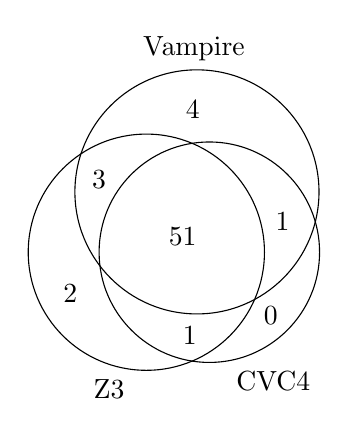
\begin{tikzpicture}
    \draw (0,0) circle (1.5cm);
    \draw (50:1cm) circle (1.55cm);
    \draw (0cm:0.8cm) circle (1.4cm);
    \node at (0.8cm:0.5cm) {$51$}; %
    \node at (-2.2cm:1.2cm) {$1$};
    \node at (1cm:-1.1cm) {$2$};
    \node at (-2cm:-1.1cm) {$3$};
    \node at (-3.8cm:-1.9cm) {$4$}; %
    \node at (-0.95cm:1.775cm) {$0$}; %
    \node at (0.45cm:1.775cm) {$1$}; %
    \node at (2.7cm:2.65cm) {Vampire};
    \node at (-3.7cm:1.8cm) {Z3};
    \node at (-1.6cm:2.3cm) {CVC4};
  \end{tikzpicture}
  \vspace{-0.3em}
  \caption{Venn diagram of the subsets of the algebraic datatypes problems, solved by Vampire, CVC4 and Z3.}
  \label{fig:smt-lib-diagram}
\end{figure}

\newcommand{\timeout}{---}
\newcommand{\gaveup}{---}
\begin{table}[tb]
  \caption{Runtimes in seconds of provers on selected algebraic datatypes problems. Dashes mean the solver failed to find a solution.}% \nofoolVampire\ denotes Vampire with disabled FOOL paramodulation.}
  \begin{center}
  \begin{tabular}{lrrr}
    \hline Problem & Vampire & CVC4 & Z3 \\ \hline
    \verb'afp/abstract_completeness/1830522' & \timeout & \timeout & 0.172 \\
    \verb'afp/bindag/2193162' & \timeout & \gaveup & 0.388 \\
    \verb'afp/coinductive_stream/2123602' & \timeout & 0.373 & 0.101 \\
    \verb'afp/coinductive_stream/2418361' & 3.392 & \timeout & \timeout \\
    \verb'afp/huffman/1811490' & 0.023 & \gaveup & \timeout \\
    \verb'afp/huffman/1894268' & 0.025 & \gaveup & 0.052 \\
    \verb'distro/gram_lang/3158791' & 0.047 & 0.179 & \timeout \\
    \verb'distro/koenig/1759255' & 0.070 & \timeout & \timeout \\
    \verb'distro/rbt_impl/1721121' & 4.523 & \timeout & \timeout \\
    \verb'distro/rbt_impl/2522528' & 0.853 & \gaveup & 0.064 \\
    \verb'gandl/bird_bnf/1920088' & 0.037 & \timeout & 0.077
  \end{tabular}
  \end{center}
  \label{table:smt-lib-nontrivial}
\end{table}

Based on our experimental results shown in Tables~\ref{table:smt-lib-results} and \ref{table:smt-lib-nontrivial}, we make the following observations. On the given set of problems the implementation of FOOL reasoning in Vampire was efficient enough to compete with state-of-the-art SMT solvers. This is significant because the problems were tailored for SMT reasoning. Vampire not only solved the largest number of problems, but also yielded runtime results that are comparable with those of CVC4. Whenever successful, Z3 turned out to be faster than Vampire; we believe this is because of the sophisticated preprocessing steps in Z3. Improving FOOL preprocessing in Vampire, for example for more efficient CNF translation of FOOL formulas, is an interesting task for further research. We note that the usage of FOOL paramodulation showed improvement.